\chapter{Conception and Realisation}
\label{chapter:conception}

\section{Literature and basics}
At the beginning, it was necessary to acquire some basics about quantum mechanics (density matrix, Maxwell-Bloch equations..) by reading some introductory literature ~\cite{tang2005}. A concrete example for the simulation and the numerical solving of the Maxwell-Bloch system was described in the paper of Ziolkowski.\\
QuTiP, a Python Toolbox for simulating the dynamics of open quantum systems, was then the starting point. It offered a variety of examples using Jupyter Notebooks: an interactive tool designed to display neatly arranged code blocks with human-friendly text which makes project easier to manage and share, they are used in this case to describe quantum mechanic systems, such as single-atom lasing, quantum Monte Carlo trajectories...\\
\section{Python/C++ Interface}
Creating the Python/C++ Interface was possible through different means:\\
\begin{itemize}
\item Boost.Python: Boost.Python is an open source C++ library which provides an interface for binding C++ classes and functions to Python. But it is bound to GCC which leads to a huge dependance and its extensive use of C++ template can cause compilation problems and the consumption of a large amount of memory. \\
\item ctpyes: ctypes is a foreign library for Python, that allows calling DLLs or shared libraries and wrapping them in Python modules. It is a convenient way to reach for a few functions within a DLL, but not to make large C++ libraries available to Python in performance-critical situations.\\
\item SWIG (Simplified Wrapper and Interface Generator): It is a language neutral compiler that turns C/C++ declarations into scripting language interfaces. It targets Python, Tcl, Perl, MATLAB, etc.. One of its important features is that it is simple and completely automated. In fact, it creates two different files; a C/C++ source file (module\textunderscore name)\textunderscore wrap.c or (module\textunderscore name)\textunderscore wrap.cxx and a Python source file (module\textunderscore name).py. The first one needs to be compiled and linked with the rest of the C/C++ library to create an extension module. The second one is the file that will be imported in Python(see Fig.\ref{fig:swig}).\\
\begin{figure}[htb]
  \centering
  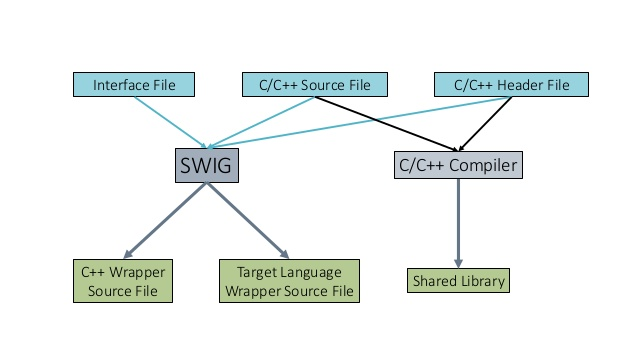
\includegraphics[width=0.5\textwidth]{figures/swig_func}
  \caption{Functionality of SWIG} ~\cite{swig}
  \label{fig:swig}
\end{figure}
\end{itemize}
After installing SWIG, a Python module was created starting from an interface file and a header file written in C++. The next step was to wrap a C++ class in order to create instances of this class and modify its attributes in the Python Testprogram. Then the complete C++ library was gradually elaborated, adding each time required attributes and declarations.\\
\section{Serialisation of input parameters}
The next point to handle was the input parameters, how to extract them from an XML File and then store them with results at the end. The first option was to use exml or lxml libraries, which could parse XML files but the resulting objects having NoType made handling them problematic. Therefore, a simple object-XML mapper for Python called dexml was applied to serialize the metadata by defining subclasses of the class dexml.Model and saving the parameters as instances.\\
\section{Storing results}
Furthermore, it was necessary to specify the file format for the simulation results, which lead to the following options:\\
\begin{itemize}
\item XML (Extensible Markup Language): XML's biggest advantage is that it provides developers with a tool that concisely and unambiguously defines the format of data records. However it is not suitable for large amount of data.\\
\item VTK (Visualization Toolkit): It is a powerful tool to visualize scalars, vectors, complex numbers.. but  requires a diffcult setup and an understanding of the framework.\\ 
\item HDF5 (Hierarchical Data Format): HDF5 is a file format that enables the storage and management of data of different types. It is suitable for high volume and complex data. In fact, a HDF5 file consists of datasets (multidimensional arrays) and groups, which contain diverse data: datasets, graphics, other groups.. Another advantage is the ability of compression and chunking, which makes the storage more flexible and efficient ~\cite{hdf5}.\\ 
\end{itemize}
All that considered, HDF5 is the most suitable file format not only to store large amount of data (results) but also different types simultaneously (Metadata).
\section{Git}
After settling the C++ library that contains all the necessary classes and functions, using SWIG to incorporate it in Python, choosing dexml for serialisation of metadata and HDF5 for storage of results, a Git project was created to gather all the pieces, register every step of the realisation and facilitate data exchange and work coordination between me and my supervisor. \\
\section{Makefile/CMake}
To get more experience in handling scientific projects, it was extremely efficient to understand the process of Makefiles and then CMake and apply them on my work. both aim at building executable programs starting from many modules.
\begin{itemize}
\item Makefiles are a simple way to organize code compilation, they consist of a list of target entries, where it is specified for each target the dependencies needed as well as the command line to apply. Besides it only rebuilds in case of new modules added to the program.
\item CMake is a cross platform build system, that automatically generates Makefiles using the CMakeListst.txt file, that specifies the packages, libraries, source files,.. needed to build.
\end{itemize}  
